\section{Overview}
\label{sec:overview}

\newcommand{\xargs}[4]{\ensuremath{[#1, #2, #3, #4]}}
\newcommand{\xform}[2]{\ensuremath{\T{xform}(#1,\ #2)}}
\newcommand{\rep}[3]{\ensuremath{\T{repeat}(#1,\ #2,\ #3)}}
\newcommand{\comb}[2]{\ensuremath{\T{combine}(#1,\ #2)}}

\newcommand{\scale}[2]{\ensuremath{\T{scale}(#1,\ #2)}}
\newcommand{\repRot}[3]{\ensuremath{\T{repRot}(#1,\ #2,\ #3)}}
\newcommand{\rotate}[2]{\ensuremath{\T{rotate}(#1,\ #2)}}
\newcommand{\translate}[3]{\ensuremath{\T{translate}(#1,\ #2,\ #3)}}

\newcommand{\pSide}[1]{\ensuremath{\T{side}(#1)}}
\newcommand{\ngon}[1]{\ensuremath{\T{ngon}(#1)}}
\newcommand{\scaledHex}[1]{\ensuremath{\T{scaledHexagon}(#1)}}

%\newcommand{\scale}[2]{\xform{#1}{\xargs{#2}{0}{0}{0}}}
%\newcommand{\rotate}[2]{\xform{#1}{\xargs{1}{#2}{0}{0}}}
%\newcommand{\translateX}[2]{\xform{#1}{\xargs{1}{0}{#2}{0}}}
%\newcommand{\translateY}[2]{\xform{#1}{\xargs{1}{0}{0}{#2}}}
%\newcommand{\translate}[3]{\xform{#1}{\xargs{1}{0}{#2}{#3}}}

%\newcommand{\scale}[2]{\ensuremath{\T{scale}\ #1\ #2}}
%\newcommand{\rot}[2]{\ensuremath{\T{rotate}\ #1\ #2}}
%\newcommand{\translX}[2]{\ensuremath{\T{translateX}\ #1\ #2}}
%\newcommand{\translY}[2]{\ensuremath{\T{translateY}\ #1\ #2}}
%\newcommand{\transl}[3]{\ensuremath{\T{translate}\ #1\ (#2, #3)}}

%In this section we illustrate our approach using a running example
%that builds upon \autoref{fig:polygons} from the introduction.

We illustrate LLMT via a running example building on \autoref{fig:polygons}.
%
The input corpus in \autoref{fig:polygons} is written in a \cogsci DSL by \citet{cogsci-dataset},
which features the following primitives:

\vspace{0.25em}
\begin{tabular}{rl}
  \T{line} &
    a line segment from
    the origin (0, 0) to the point (1, 0)
    \\
  \comb{F_1}{F_2} &
    the union of figures $F_1$ and $F_2$
    \\
  \xform{F}{\tau} &
    applying transformation $\tau$ to figure $F$
    \\
  \rep{F}{0}{\tau} &
    the empty figure
    \\
  \rep{F}{n+1}{\tau} &
    \comb{F}{\xform{\rep{F}{n}{\tau}}{\tau}}, similar to a ``fold''
\end{tabular}
\vspace{0.25em}

%%  \begin{itemize}
%%    \item
%%      \T{line} denotes
%%        a line segment from
%%        the origin (0, 0) to
%%        the point (1, 0)
%%    \item
%%      \comb{F_1}{F_2} denotes
%%        the union of figures
%%        $F_1$ and $F_2$
%%    \item
%%      \xform{F}{\tau} denotes
%%        applying transformation $\tau$
%%        to figure $F$
%%    \item
%%      \rep{F}{0}{\tau} denotes
%%        the empty figure
%%    \item
%%      \rep{F}{n+1}{\tau} denotes
%%        \xform{\comb{F}{\rep{F}{n}{\tau}}}{\tau}
%%  \end{itemize}

A transformation $\tau$ is a 4-tuple
  $\xargs{s}{\theta}{t_x}{t_y}$ denoting
  uniformly scaling by a factor of $s$,
  rotating by $\theta$ radians, and
  translating by $(t_x,\ t_y)$ in the
  $x$ and $y$ directions respectively.
% Using these,
%   \autoref{fig:polygons} features several hexagons,
%   scaled by various values of $s$,
%   implemented as:
For example, the green hexagon in \autoref{fig:polygons} is implemented as:
%
% \vspace{-1em}
\[
  \xform{
    \rep{
      \xform{
        \T{line}
      }{
        \xargs{1}{0}{-0.5}{0.5 / \tan(\pi / 6)}
      }
    }{6}{
      \xargs{1}{2\pi/6}{0}{0}
    }
  }{
    \xargs{2}{0}{0}{0}
  }
\]
%
That is, a hexagon side $\xform{\T{line}}{\xargs{1}{0}{-0.5}{0.5 / \tan(\pi / 6)}}$
is repeated six times, each time rotated by another $2\pi/6$ radians,
and the resulting unit hexagon is scaled by $2$.

% \noindent
% That is a bit unwieldy,
%   but we can easily simplify
%   by introducing a handful of
%   reusable abstractions:
% %For presentation only,
% %  we also use a handful of ``macros''
% %  to concisely describe examples in this section:

% \vspace{-0.75em}
% \[ \begin{array}{rcl}
%   \repRot{F}{n}{\theta} &=&
%     \rep{F}{n}{\xargs{1}{\theta}{0}{0}}
%     \\
%   \pSide{n} &=&
%     \xform{\T{line}}{\xargs{1}{0}{-0.5}{0.5 / \mathit{tan}(\pi / n)}}
%     \\
%   \ngon{n} &=&
%     \repRot{\pSide{n}}{n}{2\pi/n}
%     \\
%   \scale{F}{s} &=&
%     \xform{F}{\xargs{s}{0}{0}{0}}
%     \\
%   \scaledHex{s} &=&
%     \scale{\ngon{6}}{s}
% \end{array} \]

%%  \begin{itemize}
%%    \item
%%      \scale{F}{s} =
%%        \xform{F}{\xargs{s}{0}{0}{0}}
%%
%%    \item
%%      \repRot{F}{n}{\theta} =
%%        \rep{F}{n}{\xargs{1}{\theta}{0}{0}}
%%
%%    \item
%%      \pSide{n} =
%%        \xform{\T{line}}{\xargs{1}{0}{-0.5}{0.5 / \mathit{tan}(\pi / n)}}
%%
%%  \end{itemize}

%%\noindent
%%Note that our macro \pSide{n}
%%  sets up the side of a regular $n$-sided polygon
%%  by translating the unit line segment so that
%%  \repRot{\pSide{n}}{n}{2\pi/n} generates
%%  a regular $n$-sided polygon.

% \noindent
% But which of these abstractions are sufficiently useful to
%   justify including them in a library?
% The answer depends on how often they may be used
%   throughout a representative corpus of programs.
% Library learning seeks to answer this question
%   for a given corpus by synthesizing a library
%   that provides the best compression of the corpus.
% Unfortunately, this task can be complicated
%   by library function candidates
%     depending on other candidates,
%   and by seemingly trivial syntactic details.

Taking a closer look at
  the two blue hexagons in \autoref{fig:polygons},
  however, we notice something peculiar.
The two occurrences of 
\xform{\T{repeat} \ldots}{\xargs{1}{0}{0}{0}}
  % \scale{\T{repeat}(\ldots)}{1}
  in \autoref{fig:polygons} are no-ops:
  % \footnote{
  %   We use the shortened forms like ``\T{scale}''
  %   in the text merely for concision;
  %   they are fully expanded in both the
  %   corpus from~\cite{cogsci-dataset} and
  %   in \autoref{fig:polygons}.
  % }:
  they merely scale a figure $F$ by a factor of 1
  and neither rotate nor translate it.
%
These redundant transformations would likely not be there
had the code been written by hand 
or decompiled from a lower-level representation (by a tool like \tname{Szalinski}~\cite{szalinski});%
  \footnote{
    We suspect that these transformations
    ended up in the dataset of~\citet{cogsci-dataset}
    because it was generated programmatically from
    human-designed abstractions, such as ``scaled polygon''.}
and yet, they are crucial
  if we hope to learn the optimal abstraction $f_0$
  with a purely syntactic technique.

\autoref{fig:llmt} shows a simplified and ``more natural''
  version of the corpus from \autoref{fig:polygons},
  which eliminates these no-op transformations.
As illustrated in the figure,
  this causes a purely syntactic technique
  to learn a different function, $f_1$,
  which abstracts over an \emph{unscaled} unit polygon.
Because
  the scaling transformation
  is now outside the abstraction,
  it must be repeated five times.
As a result,
  although the simplified input corpus C from \autoref{fig:llmt}
  is \emph{smaller} than the original corpus A (196 AST nodes instead of 208),
  its compressed version D is \emph{larger} (81 AST nodes instead of 72)!
In other words,
  syntactic library learning is not robust
  with respect to semantics-preserving code variations.
  % This seems counterintuitive;
%   it may be difficult to explain to a
%   user why sprinkling no-ops throughout
%   code would improve learned library quality.

\begin{figure}
  \centering
  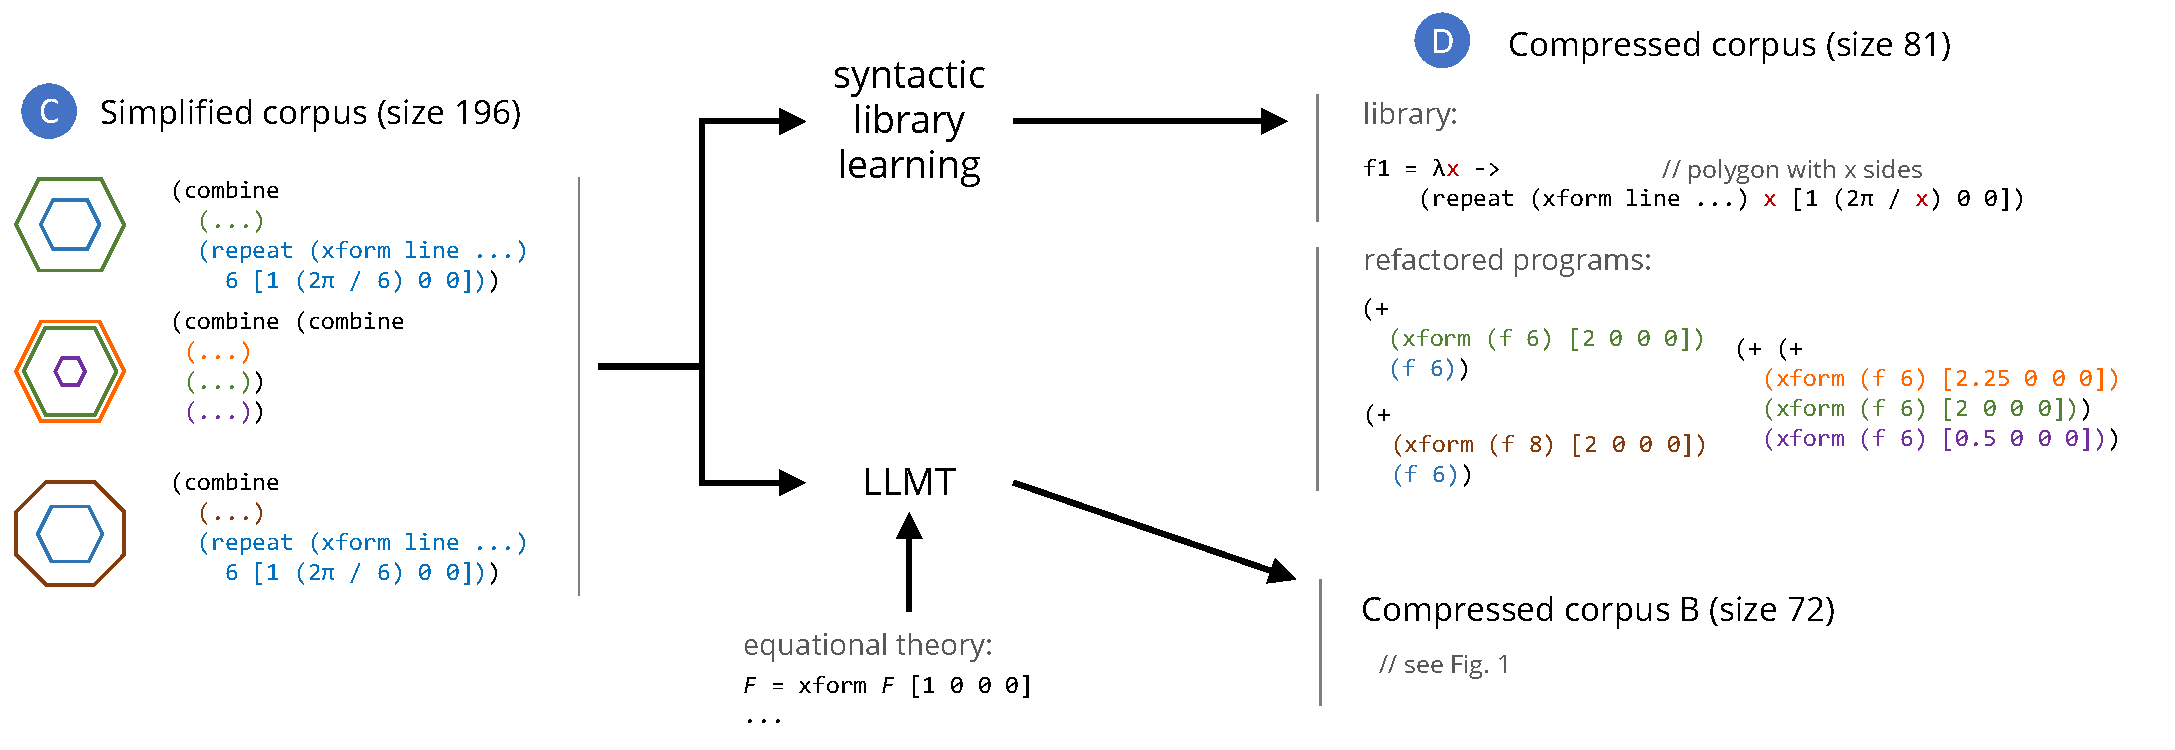
\includegraphics[width=\textwidth]{figures/polygons-simplified.pdf}
  \caption{Difference between syntactic library learning and LLMT.
           Here the initial corpus C is the simplified version of corpus A from \autoref{fig:polygons},
           with the redundant transformations on the blue subterms removed
           (unchanged terms are shown as ellipses).
           With this modification, syntactic techniques would learn an inferior abstraction $f_1$,
           leading to corpus D,
           while LLMT still learns the better abstraction $f_0$.
   }\label{fig:llmt}
\end{figure}

In contrast, our tool \tool
  can take the simplified corpus C as input
  and still discover, in a fraction of a second,
  the scaled polygon abstraction $f_0$,
  yielding the compressed corpus B of size 72.
%
In the rest of this section,
  we illustrate how \tool achieves this using our new algorithm,
  \emph{library learning modulo equational theory} (LLMT).

\mypara{Simplified DSL}
%
In the rest of this section 
  we use a tailored version of the \cogsci DSL
  with the following additional constructs:

  \vspace{0.25em}
  \begin{tabular}{rl}
    \scale{F}{s} &
      scale $F$ by a factor of $s$
      \\
    \repRot{F}{n}{\theta} &
      a special case of \T{repeat} that only performs rotation between iterations
    \\
    \pSide{n} &
      a side of a regular unit $n$-gon
  \end{tabular}
  \vspace{0.25em}

\noindent
These are expressible in the original DSL,
  and could be even discovered with library learning,
  given an appropriate corpus;
  we treat them as primitives here
  for the sake of simplifying presentation.
  

\subsection{Representing Equivalent Terms with E-Graphs}

To exploit equivalences during library learning,
%  (like a human would do),
  \tool takes as input a domain-specific equational theory.
%To be able to reason about semantics-preserving transformations like the human programmers do,
%\tool takes as input a domain-specific equational theory.
%
For our running example,
  let us assume that the theory contains a single equation:
\begin{equation}
  F \semeq \scale{F}{1} \label{eq:unit-xform}
\end{equation}
  which stipulates that any figure $F$
  is equivalent to itself 
  % transformed
  % by the no-op scaling $\T{xform}$ as described above.
  scaled by one.
%
With this equation in hand,
  it is possible to ``rewrite'' corpus C into corpus A,
  and from there learn the optimal compressed corpus B
  by purely syntactic techniques.
%
The challenge
  is that there are infinitely many
  alternative corpora C may be rewritten to;
  how do we know which to pick to maximize syntactic alignment,
  and thus the chance of discovering an optimal abstraction?

Instead of trying to guess
  the best equivalent corpus
  or enumerating them one by one,
  \tool uses \emph{equality saturation}~\cite{tate2009equality,willsey2021egg}.
%
Equality saturation takes as input
  a term $t$ and a set of rewrite rules,
  and finds the space of all terms equivalent
  to $t$ under the given rules;
  this is possible due to the high degree of
  sharing provided by the \emph{e-graph} data structure,
  which can compactly represent the resulting space.

\autoref{fig:egraph} (left) shows the e-graph
  built by equality saturation for the blue term in \autoref{fig:llmt}---%
  represented in the simplified DSL as \repRot{\pSide{6}}{6}{2\pi/6}---%
  using the rewrite rule \eqref{eq:unit-xform}.
%
The blue part of the graph represents the original term,
  and the gray part is added by equality saturation.
%
The solid rectangles in the e-graph denote
  \emph{e-nodes} (which are similar to regular AST nodes),
  while the dashed rectangles denote
  \emph{e-classes} (which represent equivalence classes of terms).
%
Importantly,
  the edges in the e-graph go from e-nodes to e-classes,
  which enables compact representation of
  programs with variation in sub-terms:
  for example, making e-class $c_1$
  the first child of the \T{repRot} node,
  enables it to represent both terms
    \repRot{\pSide{6}}{6}{2\pi/6}
%    \rep{{\color{orange}\T{line}}}{6}{\xargs{1}{2\pi/6}{0}{0}}
  and
    \repRot{\scale{\pSide{6}}{1}}{6}{2\pi/6}
%    \rep{{\color{orange}\scale{\T{line}}{1}}}{6}{\xargs{1}{2\pi/6}{0}{0}}
  without duplicating their common parts.
%
Furthermore, because e-graphs can have cycles,
  they can also represent infinite sets of terms:
  for example, the e-class $c_1$ represents
  all terms of the form:
  \pSide{6},
  \scale{\pSide{6}}{1},
  \scale{\scale{\pSide{6}}{1}}{1},
  etc.
%
Because this e-graph represents
  the space of \emph{all} equivalent terms
  up to the rewrite~\eqref{eq:unit-xform},
  the term we seek for library learning, namely
    \scale{\repRot{\pSide{6}}{6}{2\pi/6}}{1},
    %\scale{\repRot{\pSide{6}}{6}{2\pi/6}}{1},
    %\scale{\rep{\T{line}}{6}{\xargs{1}{2\pi/6}{0}{0}}}{1}
  is also represented in the e-class $c_0$.

  \begin{figure}
    \begin{minipage}{.4\textwidth}
      \centering
      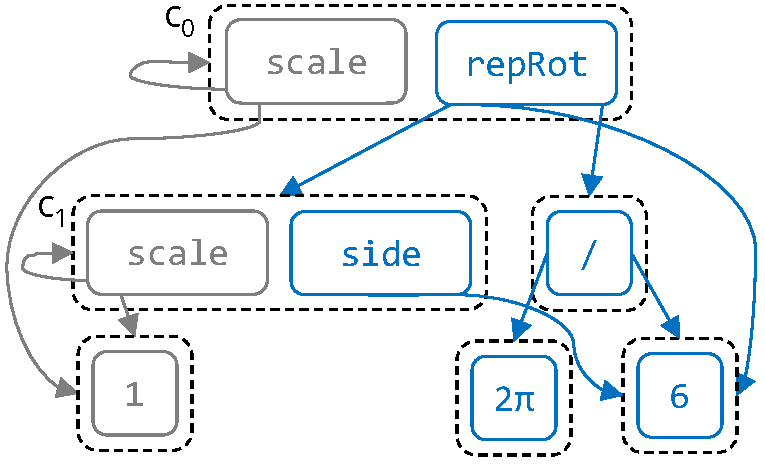
\includegraphics[width=.95\textwidth]{figures/egraph-blue.pdf}
    \end{minipage}\vline%
    \begin{minipage}{.6\textwidth}
      \centering
      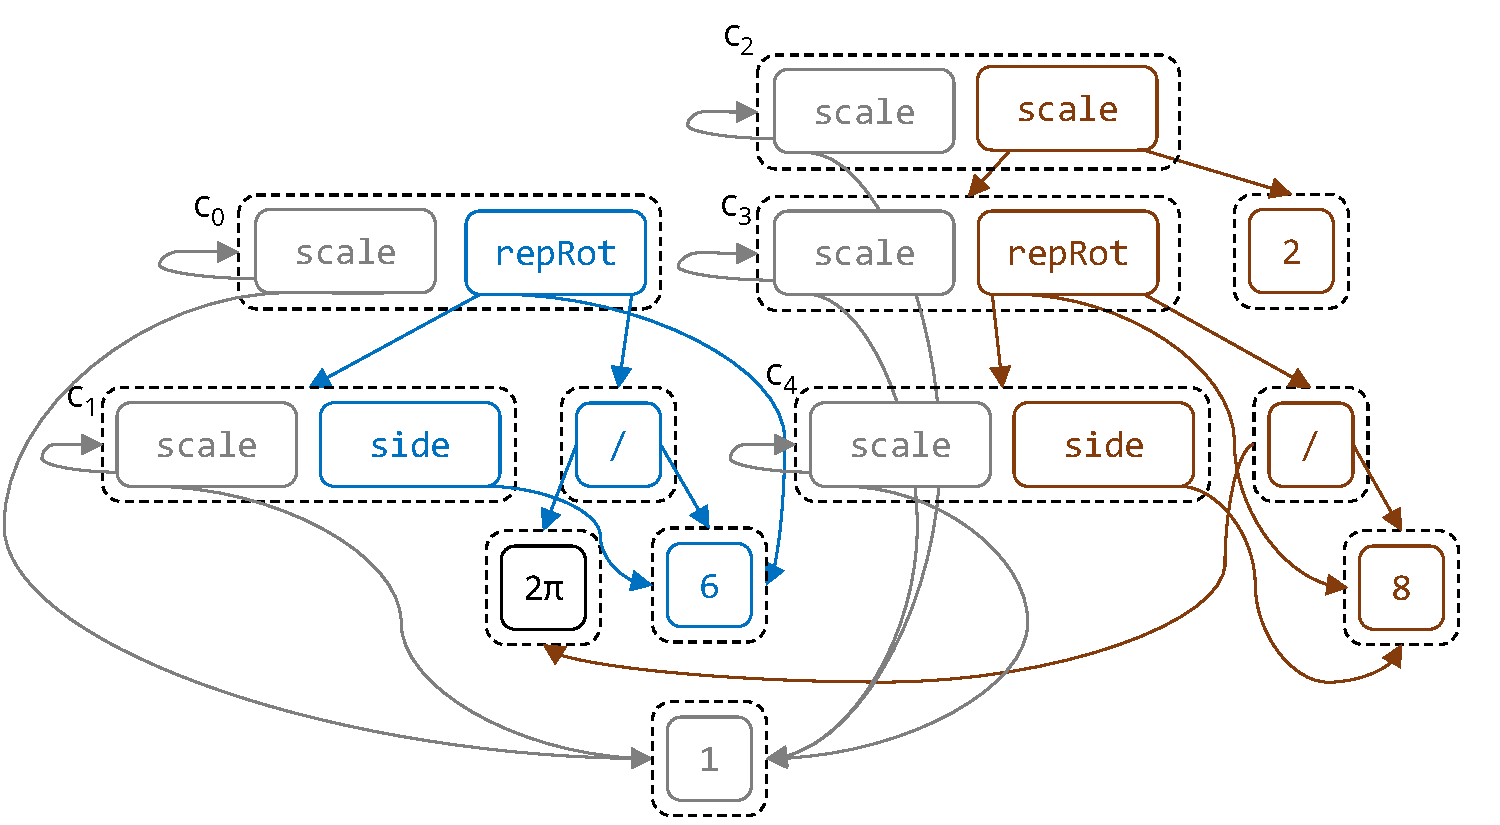
\includegraphics[width=.95\textwidth]{figures/egraph-new.pdf}
    \end{minipage}
    \caption{(Left) An e-graph representing the space of all programs
    equivalent the blue term in \autoref{fig:llmt} under rule \eqref{eq:unit-xform}.
    %
    (Right) An e-graph with both the blue and the brown terms from \autoref{fig:llmt}
    after equality saturation.
    %
    All terms are written in the simplified DSL.
    }\label{fig:egraph}
  \end{figure}  

\subsection{Candidate Generation via E-Graph Anti-Unification}

After building an e-graph from the given corpus by
  running equality saturation with the given equational theory,
  the next step in library learning is
  to generate candidate patterns
  that capture syntactic similarities across the corpus.
%\TODO{Idk if ``saturated corpus'' is a good name, because we don't necessaily reach saturation,
%but we need a name for the result of running eqsat on the original corpus.}
%
The challenge is to generate
  sufficiently few candidates
  to make library learning tractable,
  but sufficiently many to achieve good compression.
  % without missing viable candidates
  % that provide optimal compression.
We illustrate candidate generation
  using the e-graph in \autoref{fig:egraph} (right),
  which represents the part of our corpus
  consisting of the (saturated) blue and brown terms.
Recall that the optimal
  pattern---which corresponds to the scaled polygon abstraction $f_0$---is:
\begin{equation}
  P_0 = \scale{\repRot{\pSide{X}}{X}{2\pi/X}}{Y}\label{eq:p0}
  %P_0 = \T{xform (repeat line $\ X\ $ (2pi/$X$)) $\ Y$}\label{eq:p0}
\end{equation}

Prior work on \dc generates patterns by
  picking a random fragment from the corpus,
  and then replacing arbitrarily chosen subterms
  with pattern variables.
For example, to generate the pattern $P_0$,
  \dc needs to pick the entire brown subterm as a fragment,
  and then decide to abstract over its subterms $8$ and $2$.
This approach successfully restricts
  the set of candidates from
  all syntactically valid patterns
  to only those that have
  at least one match in the corpus;
  however, since there are too many ways
  to select the subterms to abstract over,
  this space is still too large to explore exhaustively
  beyond small corpora of short programs.
  % it still produces too many patterns and
  % does not scale beyond small corpora of short programs.
In \tool, this problem
  is exacerbated by equality saturation,
  since the e-graph often contains exponentially or
  infinitely more programs than the original corpus.
%since the saturated corpus often contains exponentially or infinitely more programs than the original corpus.

\mypara{Generality Filters}
%\mypara{Inviable Patterns}
%
To further prune the set of viable candidates in \tool,
  we identify two classes of patterns that can be safely discarded,
  either because they are
  too concrete or too abstract.
%
First,
  a pattern like
    \repRot{\pSide{8}}{X}{2\pi/8}
    %\T{repeat line $\ X\ $ (2pi/8)}
  can be discarded because it is
  \emph{too concrete} for this corpus:
  the corresponding abstraction
  can be applied only once,
  essentially replacing the sole matching term,
    \repRot{\pSide{8}}{8}{2\pi/8}
    %\T{repeat line 8 (2pi/8)},
  with
    $(\lambda x \bnd \rep{\pSide{8}}{x}{2\pi/8})\ 8$,
   %\T{let f = \\x->repeat line x (2pi/8) in f 8},
  which only adds more AST nodes to the corpus. % we only count vars and apps, but not lambdas, but I don't want to say it here
  %only makes the situation worse
  % by \emph{adding} three AST nodes to the corpus:
    % a $\lambda$,
    % a \T{let}-binding, and
    % an application.
%
% \TODO{There is a subtlety here: we can't say this pattern only matches a single subterm in this corpus,
% because e-class $c_2$ represents infinitely many terms, and each has a subterm that matches this pattern.
% But these terms cannot occur in the corpus simultaneously, they are alterntives, hence this pattern is still out.
% This is what our co-occurrence analysis does.
% But I think we'll talk about this in the technical section.}
%
Second,
  a pattern like
    \repRot{\pSide{X}}{X}{Y}
    %\T{repeat line $\ X\ Y$}
  can be discarded because
  it is \emph{too abstract} for this corpus:
  everywhere it matches,
  a more concrete pattern
    \repRot{\pSide{X}}{X}{2\pi/X}
    %\T{repeat line $\ X\ $ (2pi/$X$)}
  would also match;
  using the more concrete pattern
  leads to better compression,
  since the actual arguments in its applications
  are both fewer and smaller:
    \T{f 6 2pi/6} and \T{f 8 2pi/8} vs.
    \T{f 6} and \T{f 8}.

Thus,
  our \emphbf{first key insight} is 
  to restrict the set of candidates
  to the most concrete patterns that match some pair
  % that
  % any optimal candidate pattern must be the most concrete pattern
  % that matches some tuple\footnote{
  %   Note that just matching \emph{pairs} of subterms is insufficient.
  %   \TODO{ADD EXAMPLE}
  % }
  of subterms in the (saturated) corpus.%
  \footnote{As we discuss in \autoref{sec:au} this can in theory eliminate optimal patterns,
  but our evaluation shows that it works well in practice.}
%\TODO{THIS IS NOT TRUE! This should be a tuple of subterms, not pair,
%but \tool actually only does pairs; see comments about subsumption lattice in Slack; what to do???}
%
For example, pattern $P_0$
  is the most concrete pattern that matches the two terms
  \begin{gather}
    \scale{\repRot{\pSide{6}}{6}{2\pi/6}}{1}\label{eq:hex}\\
    \scale{\repRot{\pSide{8}}{8}{2\pi/8}}{2}\label{eq:oct}
    %\T{xform (repeat line 6 (2pi/6)) 1}\label{eq:hex}\\
    %\T{xform (repeat line 8 (2pi/8)) 2}\label{eq:oct}
  \end{gather}
  represented in \autoref{fig:egraph} by the e-classes $c_0$ and $c_2$, respectively.
%
% You might think this observation is too strong:
% if we consider the most concrete pattern that matches green and blue, we would discover a hexagon;
% but this is okay, because by matching every pair of subterms we will also match brown and blue,
% and discover a generic polygon.

\mypara{Term Anti-Unification}
%
Computing the most concrete pattern that
  matches two given terms is known as
  \emph{anti-unification} (AU)~\cite{Reynolds1969TransformationalSA,plotkin1970lattice}.
AU works by
  a simple top-down traversal of the two terms,
  replacing any mismatched constructors by pattern variables.
For example,
  to anti-unify the terms \eqref{eq:hex} and \eqref{eq:oct},
  we start from the root of both terms;
  since both AST nodes share the same constructor \T{scale}, %\T{xform},
  it becomes part of the pattern and we recurse into the children.
We eventually encounter a mismatch, where
  the term on the left is \T{6} and
  the term on the right is \T{8};
  so we create a fresh pattern variable $X$ and
  remember the \emph{anti-substitution}
  $\sigma = \{(\T{6}, \T{8}) \mapsto X\}$.
When we encounter a mismatch
  in the denominator of the angle,
  we look up the pair of mismatched terms
  $(\T{6}, \T{8})$ in $\sigma$;
  because we already created a variable for this pair,
  we simply return the existing variable $X$.
The final mismatch is $(\T{1}, \T{2})$
  in the second child of \T{scale}; %\T{xform};
  since this pair is not yet in $\sigma$,
  we create a second pattern variable, $Y$.
At this point,
  the resulting anti-unifier is the pattern $P_0$~\eqref{eq:p0}.

Anti-unifying
  a single pair of terms is simple and efficient.
However,
  in LLMT we want to anti-unify \emph{all pairs of subterms}
  that can occur \emph{in any corpus} equivalent
  (modulo the given equational theory)
  to the original\footnote{
      A careful reader might be wondering if
        we need to compute infinitely many anti-unifiers
        because there might be infinitely many equivalent corpora.
      As we explain shortly,
        there are only finitely many patterns that
        are viable abstraction candidates.
    }.
Explicitly enumerating all equivalent corpora
  represented by the e-graph and then
  performing AU on each pair of subterms
  is infeasible.
Instead, \tool performs
  anti-unification directly on the e-graph.

\mypara{From Terms to E-Classes}
%
We first explain how to
  anti-unify two e-classes.
This operation takes as input a pair of e-classes and
  returns a set of \emph{dominant anti-unifiers},
  \ie a set of patterns that
    (1) match both e-classes, and
    (2) is guaranteed to include
      the best abstraction 
      among the most concrete patterns 
      that match pairs of terms represented by the two e-classes.

% Consider computing $\au(c_0, c_2)$
%   for the e-classes $c_0$ and $c_2$ in
%   the e-graph from \autoref{fig:egraph} (right).
% AU still proceeds as a top-down traversal,
%   but in this context we must
%   check whether two e-classes have
%   any constructors \emph{in common}.
% In this case they do:
%   the \T{scale} constructor occurs
%   once in $c_0$ and twice in $c_2$.
% Let us first pick the brown \T{scale} e-node from $c_2$
%   (and pair it with the only \T{scale} e-node from $c_0$).
% Recursing into the first child,
%   picking the two \T{repRot} nodes,
%   and recursing again, arrive at $\au(c_1, c_4)$
%   we now need to compute $\au(c_0, c_3)$.
% For these two e-classes,
%   let us first consider the two \T{repRot} nodes;
%   again, we recurse and arrive at $\au(c_1, c_4)$.
% Since these two e-classes have
%   a single pair of e-nodes in common (the \T{repeat} nodes),
%   we again recurse and arrive at $\au(c_1, c_1)$.

Consider computing $\au(c_1, c_4)$
  for the e-classes $c_1$ and $c_4$ in
  the e-graph from \autoref{fig:egraph} (right).
AU still proceeds as a top-down traversal,
  but in this context we must
  check whether two e-classes have
  any constructors \emph{in common}.
In this case they do:
  both a \T{side} constructor and a \T{scale} constructor.
Let us first pick the two \T{side} constructors
  and recurse into their only child,
  computing $\au(\{\T{6}\}, \{\T{8}\})$.
These two e-classes have
  no matching constructors,
  so AU simply returns a pattern variable,
  similarly to term anti-unification;
  this yields the first pattern for $c_1$ and $c_4$: $\T{side}\ X$.
  
Recall, however, that $c_1$ and $c_4$ also 
  have matching \T{scale} constructors.
This is where things get interesting:
  these constructors are involved in a \emph{cycle} 
  (their first child is the parent e-class itself).
If we let AU follow this cycle, the set of anti-unifiers becomes infinite:
  $$
    \au(c_1, c_4) = \{\T{side}\ X\} \cup \{\T{scale}\ p\ 1 \mid p \in \au(c_1, c_4)\}
  $$
Fortunately,
  we can show that $\T{side}\ X$ \emph{dominates}
  all the other patterns from this set,
  because their pattern variables---in this case, just $X$---match
  the same e-classes, but they are also larger
  (in \autoref{sec:egraphs} we show how
  this domination relation lets us prune other patterns,
  not just those caused by cycles).
Hence $\au(c_1, c_4)$ simply returns $\{\T{side}\ X\}$.
% \TODO{In fact it also returns $X$ because they have mismatched constructors as well,
% and we explain this in sec 4. Should we say this here?}

% When AU encounters two e-classes with
%   no matching constructors,
%   it introduces a pattern variable,
%   similarly to term anti-unification
%   (again, keeping tack of the anti-substitution to
%   avoid introducing redundant variables).
Following the same logic for the root e-classes of the two polygons, $c_0$ and $c_2$,
  $\au(c_0, c_2)$ yields that pattern $P_0$~\eqref{eq:p0},
  which is required to learn the optimal abstraction.
% Recall, however,
%   that $c_2$ has a second \T{xform} e-node,
%   which we also need to try.
% This, however, leads to a cycle:
%   $$
%     \au(c_0, c_2) = \{P_0\} \cup \{\T{xform}\ p\ 1 \mid p \in \au(c_0, c_2)\}
%   $$
% The cyclic solution is discarded as non-dominant,
%   for the same reason as explained above.

% \TODO{This generalized to $n$ e-classes in the ``natural way'' ?!}

\mypara{From E-Classes to E-Graphs}
%
To obtain the set of all candidate abstractions,
we need to perform anti-unification over all pairs of e-classes in the e-graph.
%
Clearly, these computations have overlapping subproblems
(for example, we have to compute $\au(c_1, c_4)$ 
as part of $\au(c_0, c_2)$ and  $\au(c_0, c_3)$).
%
To avoid duplicating work, \tool uses an efficient dynamic programming algorithm
that processes all pairs of e-classes in a bottom-up fashion.

\subsection{Candidate Selection via Targeted Common Subexpression Elimination}

We now illustrate the final step of library learning in \tool:
given the set of candidate abstractions generated by e-graph anti-unification,
the goal is to pick a subset that gives the best compression for the corpus as a whole.
%
% This is a non-trivial combinatorial search problem.
%
For example, the candidates generated for the corpus from \autoref{fig:llmt} include:
\[ \begin{array}{rcll}
%
  f_0 &=& \lambda x\ y \bnd \scale{\repRot{\pSide{x}}{x}{2\pi/x}}{y} &\quad \text{scaled regular $x$-gon} \\[2pt]
%
  f_1 &=& \lambda x \bnd \repRot{\pSide{x}}{x}{2\pi/x} &\quad \text{regular $x$-gon} \\[2pt]
%
  f_2 &=& \lambda y \bnd \scale{\repRot{\pSide{6}}{6}{2\pi/6}}{y} &\quad \text{scaled hexagon}
%
%f_0 = \T{\\x y->trans (repeat line x (2pi/x)) y} &\quad \text{scaled polygon}\\
%f_1 = \T{\\x->repeat line x (2pi/x)} &\quad \text{polygon}\\
%f_2 = \T{\\y->trans (repeat line 6 (2pi/6)) y} &\quad \text{scaled hexagon}
\end{array} \]
%
It is not immediately clear which abstraction is better:
  $f_0$ matches more terms than $f_2$,
  but $f_2$ requires fewer arguments
  (so if we have enough scaled hexagons in the corpus and
  only one octagon, it might be better to leave the
  octagon un-abstracted).
On the other hand,
  $f_1$ might be better,
  since it does not introduce the
  redundant transformation on the blue hexagons.
Finally,
  if we pick $f_0$ \emph{and} $f_2$ together,
  we can also abstract the definition of
  $f_2$ as $f_0\ 6$, thereby getting additional reuse!
As you can see,
  candidate selection is highly non-trivial,
  since it needs to take into account the
  choice between different equivalent programs in the e-graph, %saturated corpus,
  and the fact that some abstractions can be defined using others.

\begin{figure}
  \centering
  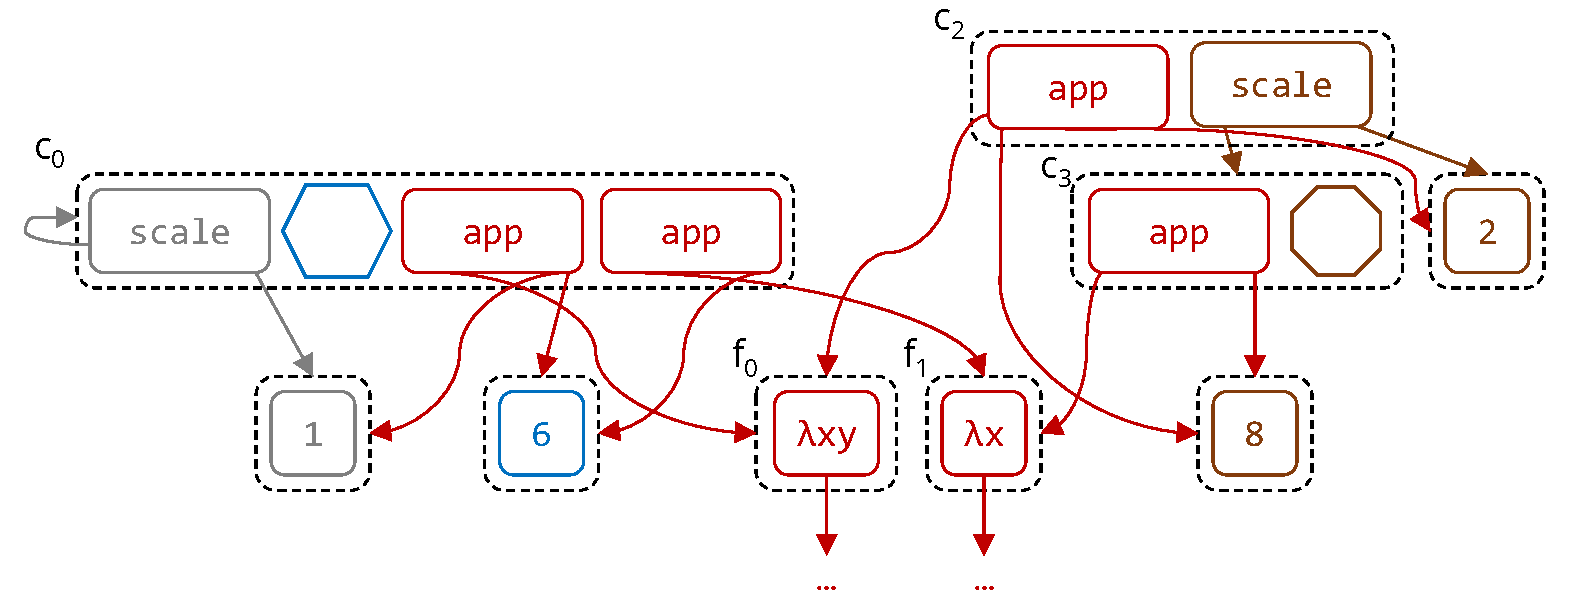
\includegraphics[width=.8\textwidth]{figures/beam.pdf}
  \caption{The e-graph from \autoref{fig:egraph} (right) with applications of $f_0$ and $f_1$ depicted in red.
           We show the unchanged parts of the graph representing the unit hexagon and octagon as corresponding shapes;
           we also omit some of the gray e-nodes added in the previous stage.}\label{fig:beam}
\end{figure}

\mypara{Reduction to E-Graph Extraction}
%
To overcome this difficulty, we once again leverage e-graph and equality saturation.
%
Our \emphbf{second key insight} is that selecting the optimal subset of abstractions
can be reduced to the problem of extracting the smallest term from an e-graph
in the presence of common sub-expressions.

To illustrate this reduction,
% let us again consider the part of the corpus depicted on \autoref{fig:egraph} (right),
% that is the saturated version of the blue and the brown polygons, and
let us limit our attention to only two candidate abstractions, $f_0$ and $f_1$, defined above.
%
\tool converts each of the candidate patterns and its corresponding abstraction into a rewrite rule
that introduces a \emph{local} $\lambda$-abstraction followed by application into the corpus;
for our two abstractions these rules are:
\begin{align}
  % \scale{\repRot{\pSide{X}}{X}{2\pi/X}}{Y} &\Rightarrow (\lambda x\ y \bnd \scale{\repRot{\pSide{x}}{x}{2\pi/x}}{y})\ X\ Y\\ 
  % \repRot{\pSide{X}}{X}{2\pi/X} &\Rightarrow (\lambda x \bnd \repRot{\pSide{x}}{x}{2\pi/x})\ X 
  \scale{\repRot{\pSide{X}}{X}{2\pi/X}}{Y} &\Rightarrow f_0\ X\ Y\label{eq:rw1}\\ 
  \repRot{\pSide{X}}{X}{2\pi/X} &\Rightarrow f_1\ X \label{eq:rw2}
\end{align}
%
The result of applying these rules to the e-graph from \autoref{fig:egraph} (right)
is shown in \autoref{fig:beam}.
%
For example, you can see that the e-class $c_2$ (which represents the scale-2 octagon)
now stores an alternative representation:
% \T{let f0 = \\x y->trans (repeat line x (2pi/x)) y in f0 2 8}.
% $\T{let}\ f_0 = \lambda x\ y \bnd \scale{\repRot{\pSide{x}}{x}{2\pi/x}}{y}\ \T{in}\ f_0\ 2\ 8$.
% $(\lambda x\ y \bnd \scale{\repRot{\pSide{x}}{x}{2\pi/x}}{y})\  2\ 8$.
$f_0\  8\ 2$.
%
The e-class $c_0$ (unit hexagon)
has representations using either $f_0$ or $f_1$,
because this class matches both rewrite rules \eqref{eq:rw1} and \eqref{eq:rw2} above. % pattern above.
%
Note also that because the definitions of the $\lambda$-abstractions are also stored in the e-graph,
equality saturation can use the above rewrite rules inside their bodies,
to make one function use another:
for example, one term stored for the definition of $f_0$ is
$$
\lambda x\ y \bnd \scale{f_1\ x}{y}.
$$

Once we have built the version of the e-graph with local lambdas for all the candidate abstractions,
all that is left is to extract the smallest term out of this e-graph.
%
The tricky part is that we want to count the size of the duplicated lambdas only once.
%
For example, in \autoref{fig:beam}, $f_0$ is applied twice (in $c_0$ and $c_2$);
if term extraction were to choose both of these e-nodes,
we want to treat their first child (the definition of $f_0$) as a common sub-expression,
whose size contributes to the final expression only once.
%
Intuitively, this is because we can ``float'' these lambdas 
into top-level \T{let}-bindings,
thereby defining $f_0$ only once, and replacing each local lambda with a name.

Extraction with common sub-expressions is a known but notoriously hard problem,
which is traditionally reduced to integer linear programming (ILP)~\cite{tensat,spores}.
%
Because the scalability of the ILP approach is very limited,
we have developed a custom extraction algorithm,
which scales better by using domain-specific knowledge and approximation.


\mypara{Extraction Algorithm}
%
The main idea for making extraction more efficient is that
for library learning we are only interested in sharing a certain type of sub-terms:
namely, the $\lambda$-abstractions.
%
Hence for each e-class we only need to keep track
of the the best term for each possible library
(\ie each subset of $\lambda$-abstractions).
%
More precisely, for each e-class and library,
we keep track of
  (1) the smallest size of the library
  (2) the smallest size of the program refactored using this library 
  (counting the $\lambda$-abstractions as a single node).
%
We compute and propagate this information bottom-up through the e-graph.
%
Once this information is computed for the root e-class
(that represents the entire corpus),
we can simply choose the library with the smallest total size.

For example, for the e-class $c_2$ from \autoref{fig:beam},
with the empty library $\emptyset$, the size of library is 0 and the size of the smallest program (\scale{\repRot{\pSide{8}}{8}{2\pi/8}}{2}) is 9;
with the library $\{f_0\}$, the size of the library is 9 and the size of the smallest program ($f_0\ 2\ 8$) is 3;
while with the library $\{f_1\}$, the size of the library is 7 and the size of the smallest program (\scale{f_1\ 8}{2}) is 4.
% For c_0: $\emptyset$ -> 6, $\{f_0\}$ -> 3, $\{f_1\}$ -> 2.
% For c_2: $\emptyset$ -> 8, $\{f_0\}$ -> 3, $\{f_1\}$ -> 4.
%
Clearly for this e-class introducing library functions is not paying off yet ($0 + 9 < 7 + 4 < 9 + 3$),
since each one can be only used once.
%
This situation changes, however, as we move up towards the root.
%
Already for the parent e-class of $c_0$ and $c_2$,
the cost of introducing $\{f_0\}$ and $\{f_1\}$ is amortized:
the size of the smallest program is 17 with the empty library and 7 with either $\{f_0\}$ or $\{f_1\}$,
so $\{f_1\}$ is already worthwhile to introduce ($9 + 7 < 0 + 17$).
%
Including even more programs with scaled polygons eventually makes the library $\{f_0\}$ the most profitable of the four subsets.

Since in a larger corpus, keeping track of all subsets of candidate abstractions is not feasible,
\tool provides a way to trade off scalability and precision
by using a \emph{beam search} approach.


% \mypara{Approximate Extraction with Beam Search}
% %
% The algorithm described so far is precise,
% but does not scale to large sets of candidate abstractions,
% since it has to track all subsets.
% %
% \tool provides a way to trade off scalability and precision
% by using a \emph{beam search} approach.
% %
% To reduce the set of libraries that needs to be stored in each e-class,
% the user can provide bounds both on
%   (1) the maximum \emph{size} of the library, and
%   (2) the maximum number of distinct best libraries considered for each e-class (\ie the \emph{beam size}).
% %
% \TODO{Should we talk about partial-order reduction here?}

